\section{\emph{rag}, a Ruby Autograder for ESaaS}

Having chosen Ruby and Rails for their excellent testing and
code-grooming tools, our approach was to repurpose those same tools into
autograders that would give finer-grained feedback than human graders
using more detailed tests, and would be easier to repurpose than
those built for other languages.

\begin{figure}
  \centering
  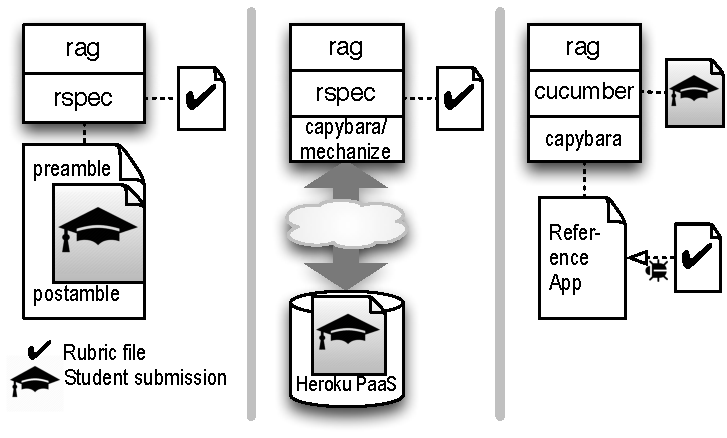
\includegraphics[width=0.7\textwidth]{figs/rag.pdf}
  \begin{tabular}{|p{0.15\textwidth}|p{0.15\textwidth}|p{0.7\textwidth}|}
 \hline
 \textbf{Grader} & \textbf{Based on} & \textbf{Student Assignment Type} \\
 \hline
 RSpecGrader &
 unit testing &
 Student submits one or more class files; black-box and ``intrusive''
 unit tests against functions and groups of functions are performed
 \\
 FeatureGrader &
 simplified mutation testing &
 Student submits integration tests written using Cucumber; bugs inserted
 in reference app attempt to trigger test failures to check test suite
 completeness and test fragility
 \\
 MechanizeGrader & 
 staging-like integration testing &
 Student deploys full-stack app to public cloud; ``black box'' tests
 stimulate remote server and parse/analyze output, including execution
 of JavaScript if needed
 \\
 \hline
\end{tabular}

  \caption{\label{fig:grader_summary} Summary of the autograder
    engines based on our repurposing of excellent existing open-source
    tools and testing techniques.  Only the RSpecGrader is
    Ruby-specific.}
\end{figure}

\texttt{rag}\uf{github.com/saasbook/rag} is actually a collection of
three different autograding ``engines'' based on open-source testing
tools, as Figure~\ref{fig:grader_summary} shows.
Each engine takes as input a student-submitted work product and one or
more rubric files whose content depends on the grader
engine\footnote{Currently the rubric files must be present in the local
filesystem of the autograder VM, but refactoring is in progress to
allow these files to be securely loaded on-demand from a remote host
so that currently-running autograder VMs do not have to be modified
when an assignment is added or changed.}, and grades the work
according to the rubric.
The first of these (Figure~\ref{fig:grader_summary}, left) is
\textbf{RSpecGrader}, based on RSpec, an XUnit-like TDD framework that
exploits Ruby's flexible syntax to embed a highly readable unit-testing
DSL in Ruby.
The instructor annotates specific tests within an assignment with point
values (out of 100 total); RSpecGrader computes the total points
achieved and concatenates and formats the error/failure messages from
any failed tests, as Figure~\ref{fig:rspec_grader_rubric} shows.
RSpecGrader wraps the student code in a standard preamble and postamble
in which large sections of the standard library such as file I/O and
most system calls have been stubbed out, allowing us to handle
exceptions in RSpec itself as well as test failures.
RSpecGrader also runs in a separate timer-protected interpreter thread
to protect against infinite loops and pathologically slow student code.

A variant of RSpecGrader is \textbf{MechanizeGrader}  (Figure~\ref{fig:grader_summary}, center).
Surveys of recent
autograders~\cite{ihantola-2010-autograding-survey,douce-2005-autograding-survey}
mentioned as a ``future direction'' a grader that can assess full-stack
GUI applications.
MechanizeGrader does this using Capybara and
Mechanize\footnote{\url{jnicklas.github.io/capybara},
\url{rubygems.org/gem/mechanize}}.
Capybara implements a Ruby-embedded DSL for interacting with Web-based
applications by providing primitives that trigger actions on a web page
such as filling in form fields or clicking a button, and examining the
server's delivered results pages using XPath\uf{w3.org/TR/xpath20/}, as
Figure~\ref{fig:mechanize_grader_example} shows. 
Capybara is usually used as an in-process testing tool, but Mechanize
can trigger Capybara's actions against a remote application, allowing
black-box testing.
Students' ``submission'' to MechanizeGrader is therefore the URL to their
application deployed on the public 
cloud.  (We use the free tier of Heroku for our assignments and
projects.)

Finally, one of our assignments requires students to write integration-level
tests using Cucumber, which allows such tests to be formulated in
stylized plain text, as Figure~\ref{fig:cucumber} shows.
Our autograder for this
style of assignment is inspired by mutation testing, a technique invented
by George Amman and Jeff 
Offutt~\cite{ammann-offutt-sw-testing} in which a
testing tool pseudo-randomly mutates the program under test to ensure
that some test fails as a result of these introduced errors.


\begin{figure}
  \begin{minipage}{0.45\textwidth}%
  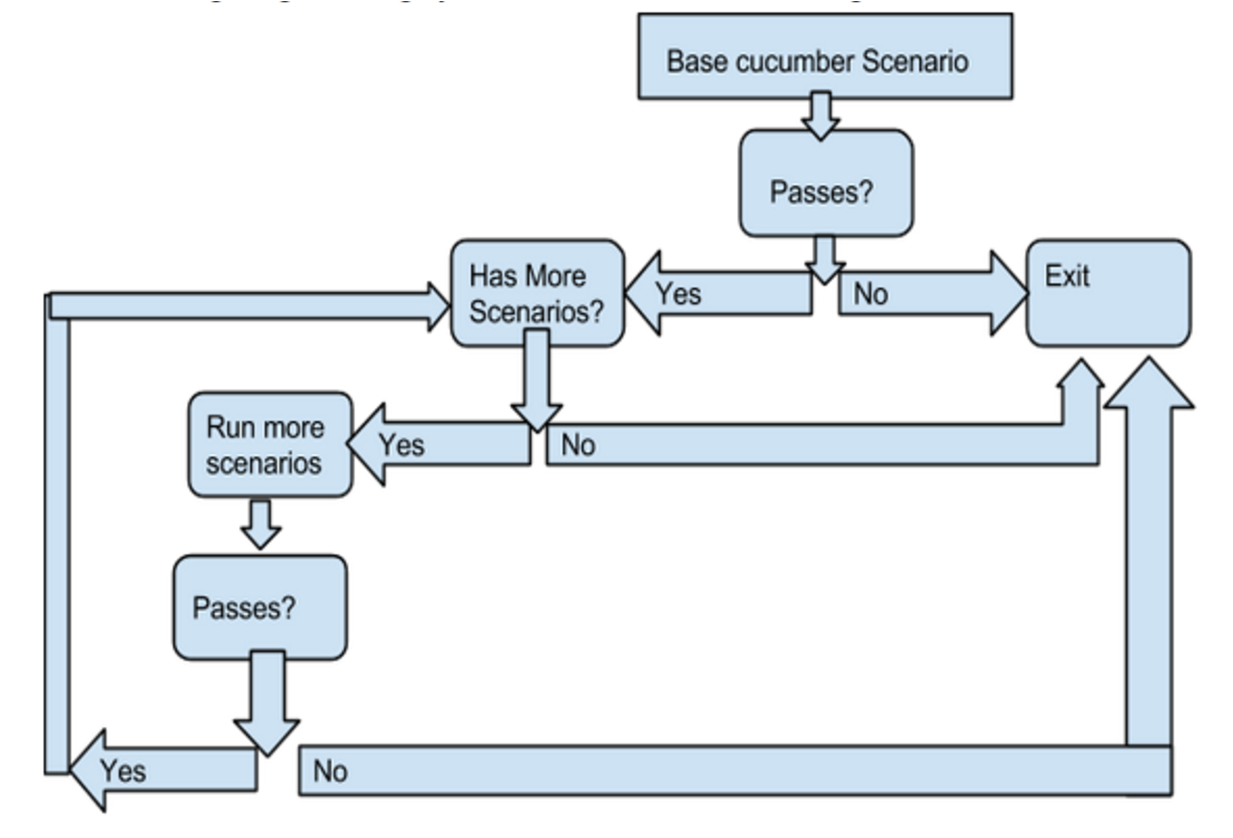
\includegraphics[width=\textwidth]{figs/feature_grader.pdf}%
  \end{minipage}%
  \begin{minipage}{0.55\textwidth}%
  \lstinputlisting{figs/feature_grader_example.yml}%
  \end{minipage}
  \caption{\label{fig:featuregrader}%
FeatureGrader workflow and example YAML file.  In this case if Step1-1 passes,
Step1-3 will be run next.  Earlier steps must be less restrictive than
later steps (if the earlier step fails, there should be no way that a later one could pass).
\texttt{failures} are the two student-provided Cucumber scenarios that \emph{should fail} when
run because of mutations (bugs) inserted in the app.
}
\end{figure}


Specifically, \textbf{FeatureGrader}  (Figure~\ref{fig:grader_summary},
right)
operates by working with an
reference application designed so that its behavior can be modified by
manipulating certain environment variables.
Each student-created test   is first applied to the reference
application to ensure it passes when run against a known-good subject.
Next the FeatureGrader starts to mutate the reference application
according to a simple specification (Figure~\ref{fig:featuregrader}), 
introducing specific bugs and checking that some student-created test
does in fact fail in the expected manner in the presence of the
introduced bug.  
